
\section{Konkrete Missbrauchsszenarien ohne ausreichende Gegenmaßnahmen}
\label{sec:szenarien}

Basierend auf den Arbeiten von Heinrich \textit{et al.} \cite{Heinrich_FindMy}, Tonetto \textit{et al.} \cite{Tonetto_FindMy}, Mayberry \textit{et al.} \cite{Mayberry_Tracking} und Garg \textit{et al.} \cite{Garg_Secure_Tracker}, sind im Folgenden sechs Missbrauchsszenarien aufgeführt, welche nicht ausreichend durch Gegenmaßnahmen unterbunden werden.
Gegen einige werden aktuell keine Maßnahmen getroffen, andere Gegenmaßnahmen lassen sich leicht umgehen und sind dementsprechend nicht ausreichend.
Neben der Erläuterung des Szenarios werden jeweils Gegenmaßnahmen vorgeschlagen, welche von Apple oder den Nutzern des Dienstes beziehungsweise den Betroffenen umgesetzt werden können.
In diesem Zusammenhang werden auch mögliche Probleme dieser Gegenmaßnahmen aufgezeigt.

Weiterhin ist Szenario \nameref{missbrauch:4} differenziert zu betrachten, da es sowohl einen negativen als auch einen positiven Missbrauch des Dienstes beschreibt.
In einem Fall lässt sich der Dienst nutzen, um die Privatsphäre Dritter einzuschränken.
Im anderen Fall erfolgt der Missbrauch, zum Schutz der Privatsphäre.
Weil dieser Anwendungsfall jedoch nicht von Apple vorgesehen ist, handelt es sich dennoch um Missbrauch.



Allgemein konnten keine Gegenmaßnahmen identifiziert werden, welche jedes der Szenarien unterbinden können.
Die Nutzer des „Wo ist?“ Dienstes können sich jedoch gegen alle Missbrauchsszenarien außer \nameref{missbrauch:3} schützen, indem sie den Dienst nicht nutzen und der Teilnahme als Finder Devices widersprechen.
Da der Dienst jedoch sehr nützlich sein kann, wird diese Gegenmaßnahme allerdings nicht als sinnvoll angesehen.
Stattdessen werden, wenn möglich, zu den jeweiligen Szenarien Gegenmaßnahmen vorgestellt, die eine möglichst uneingeschränkte Nutzung des Dienstes erlauben.


\subsection[M1]{M1: Replay-Angriff}
\label{missbrauch:1}
Durch die Ende-zu-Ende-Verschlüsselung und den authentifizierten Upload der Standortdaten, kann die Integrität der Standortdaten in vielen Fällen geschützt werden.
Allerdings können Replay-Angriffe genutzt werden, um dafür zu sorgen, dass manipulierte Standortdaten auf Apples Server und auf das Owner Device gelangen.
Diese sind korrekt verschlüsselt und werden ebenfalls korrekt authentifiziert hochgeladen, sodass für Apples Server keine triviale Möglichkeit besteht die Manipulation zu erkennen.

Durch Replay-Angriffe kann die Integrität der abgerufenen Standortdaten nicht mehr gewährleistet werden.
Der Nutzer kann bei abgerufenen widersprüchlichen Standortinformationen nicht zwischen korrekten und manipulierten Daten unterscheiden und erhält somit keine verlässlichen Standortinformationen, was die Verfügbarkeit beeinträchtigt \cite{Heinrich_FindMy}.
Dieser Angriff entspricht im wesentlichen \ac{DOS}-Angriff durch einen Angreifer in der Nähe (A2 mit Ziel (3) in \autoref{fig:adversary_models}).
Allerdings kann hier das Ziel auch in der reinen Manipulation der Standortdaten liegen, die Verfügbarkeit muss nicht in jedem Fall betroffen sein.
\begin{figure}[ht]
    \centering
    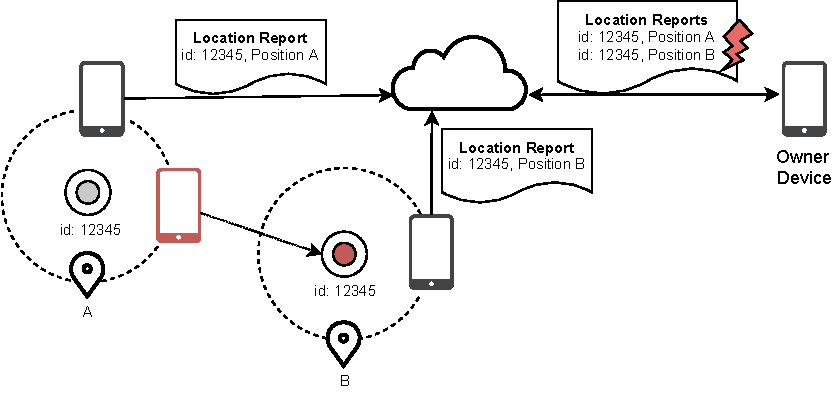
\includegraphics[width=0.9\textwidth]{replay.pdf}
    \caption{Schema eines Replay-Angriffs, um die Integrität verfügbarer Standortdaten zu beeinträchtigen.}
    \label{fig:replay_attack}  
\end{figure}

Das grundsätzliche Schema eines Replay-Angriffs ist in \autoref{fig:replay_attack} dargestellt.
Um einen solchen Angriff durchzuführen, zeichnet ein Angreifer zunächst die Advertisement-Pakete und damit den öffentlichen Advertising Key eines Lost Device auf.
Anschließend kann der Angreifer die Aufzeichnung zu einer anderen Zeit oder an einem anderen Ort senden.
Geräte in der Nähe empfangen die wiederholten Pakete und erstellen Location Reports, welche mit dem enthaltenen Advertising Key verschlüsselt werden.
Bei einer Anfrage erhält das Owner Device beispielsweise sowohl korrekte als auch manipulierte Standortdaten.
Es kann nicht bestimmt werden, welche Informationen korrekt sind, weshalb die Daten für die Lokalisierung verlorener Geräte nicht geeignet sind.

\subsubsection{Gegenmaßnahmen}
Das Design des Dienstes lässt es prinzipiell zu, Replay-Angriffe zumindest erkennen zu können.
Die „Wo ist?“ App könnte beispielsweise die Plausibilität der empfangenen Standortdaten prüfen und Nutzer auf eventuelle Manipulationen hinweisen.
Eine solche Prüfung wäre unter anderem anhand der Erstellungszeitpunkte der Location Reports möglich.
Große Abweichungen des Standorts bei Reports, welche in einem kurzen Zeitraum erstellt wurden, könnten als potenziell manipuliert erkannt werden.
Allerdings lassen sich so nicht alle Manipulationen erkennen, da der Replay-Angriff zum Beispiel auch in der Nähe des tatsächlichen Standorts durchgeführt werden kann, sodass die Abweichungen der Standorte klein sind.
In diesem Fall wird lediglich die Genauigkeit der Lokalisierung eingeschränkt.
Außerdem könnte das Owner Device bestimmen, welcher Advertising Key zum Zeitpunkt der Generierung des Location Reports aktiv war und so überprüfen ob der Location Report mit dem passenden Advertising Key erstellt wurde, oder ob ein älterer Schlüssel verwendet wurde.
So lassen sich mögliche Replay-Angriffe auf das Intervall der Schlüsselrotation beschränken.

Jedoch sind diese Maßnahmen nur durch Apple, durch eine Aktualisierung der „Wo ist?“ App umsetzbar. 
Auf Apples Server können Manipulationen hingegen nicht erkannt werden, da durch die Verschlüsselung kein Zugriff auf die Standortinformationen besteht, welche für die Prüfung der Plausibilität benötigt werden.

Die Nutzer haben keine Möglichkeit, sich vor einem Replay-Angriff zu schützen.
Sobald ein Gerät Advertisement-Pakete sendet, könnten diese von einem Angreifer aufgezeichnet und für einen Replay-Angriff verwendet werden.


\subsection[M2]{M2: \ac{DOS}: Angreifer in der Nähe}
\label{missbrauch:2}
Die Verfügbarkeit der Standortdaten ist für die Betrachtung im Rahmen dieser Arbeit weniger relevant, da das Design des Dienstes wenige Auswirkungen auf die Verfügbarkeit hat.
Dennoch ist die Verfügbarkeit durch verschiedene Angriffe bedroht.
Die Verfügbarkeit von Standortdaten lässt sich durch den Missbrauch von Funktionen des Dienstes durch einen Angreifer in \ac{BLE}-Reichweite eines Lost Device beeinträchtigen.
Dieser Angriff entspricht dem dritten Ziel des Angreifers in der Nähe (A3 mit Ziel (3) in \autoref{fig:adversary_models}).

Garg \textit{et al.} \cite{Garg_Secure_Tracker} zeigen bei einem von ihnen entwickelten Crowdsourced-Tracking Dienst, dass ein Angreifer in der \ac{BLE}-Reichweite des Geräts in der Lage ist, die Batterie des Geräts gezielt zu entladen.
Beim betroffenen System wird der aktuelle Standort vom Finder Device an das Lost Device gesendet, welches die Daten verschlüsselt zurückgibt.
Da sowohl Verschlüsselung als auch aktive \ac{BLE}-Kommunikation energieintensiv sind, kann ein Angreifer durch das häufige Anfragen der Verschlüsselung die Batterie des Geräts entladen.

Ein Angriff nach diesem Schema kann prinzipiell auch Apples System betreffen.
Insbesondere für Accessories mit üblicherweise geringer Batteriekapazität ist die gezielte Entladung ein relevantes Bedrohungsszenario.
Da jedoch beim „Wo ist?“ Dienst die Verschlüsselung nicht auf dem Lost Device erfolgt, muss der Angriff leicht variiert werden.
Laut Apples Spezifikation müssen Accessories die Möglichkeit bieten, einen Ton abzuspielen.
Diese Funktion ist Teil der \ac{UT} und soll Nutzer vor direktem Tracking, wie in \nameref{missbrauch:3} beschrieben, warnen und das Auffinden versteckter Tracker ermöglichen \cite{Apple_FindMySpec}.
Allerdings kann diese Funktion durch alle Geräte in \ac{BLE}-Reichweite missbraucht werden, um Töne abzuspielen \cite{Heinrich_AirGuard}.
Das Abspielen von Tönen ließe sich im Rahmen eines Angriffes so lange wiederholen, bis die Batterie des Lost Devices entladen ist.

\subsubsection{Gegenmaßnahmen}
Da das Abspielen eines Tons auffällig und damit für Angreifer nicht in jeder Situation geeignet ist, ist diese Art des Missbrauchs weniger praxisrelevant und Maßnahmen vermutlich nicht zwingend notwendig.
Dennoch sollen mögliche Maßnahmen vorgestellt werden.

Als Gegenmaßnahme könnte Apple die Funktion, Töne abzuspielen, entfernen.
So würde der Angriff nicht komplett verhindert, aber erschwert werden.
Allerdings ist diese Funktion Teil der Schutzmaßnahmen gegen direktes Tracking und die Entfernung dieser Funktion würde die Maßnahmen zur \ac{UT} abschwächen.


Die Nutzer haben kaum Möglichkeiten sich gegen dieses Szenario zu schützen. 
Das Entfernen des Lautsprechers von Accessories wäre eine Möglichkeit die Entladung durch Angreifer in der Nähe zu erschweren.
Da die Entladung durch das Abspielen von Tönen jedoch auffällig und demnach als eher unwahrscheinlich anzusehen ist, ist auch diese Maßnahme nur bedingt sinnvoll.


\subsection[M3]{M3: Direktes Tracking von Personen}
\label{missbrauch:3}
Das Szenario des direkten Trackings von Personen bezieht sich auf die Verfolgung durch AirTags oder andere kleine Tracker.
Durch die kleine Größe der Tracker können diese in Jacken, Rucksäcken oder an Fahrzeugen befestigt werden, um einzelne Personen gezielt zu verfolgen \cite{Roth_airtags}.
Finder Devices in der Nähe der Tracker erzeugen Location Reports, die ein Angreifer zur Bestimmung der Position der Tracker und damit der Position des Opfers abrufen kann.
Solche Angriffe wurden bereits vielfach in der Praxis beobachtet und für Stalking oder Autodiebstahl genutzt \cite{NYT_Airtags}.
Dieses Szenario lässt sich keinem der Angreifermodelle von Heinrich \textit{et al.} \cite{Heinrich_FindMy} zuordnen, da es keinen Angriff auf den Dienst, sondern ein gezielter Missbrauch des Dienstes darstellt.
Der Angreifer ist ein legitimer Nutzer des Dienstes, der ein Lost Device lokalisiert.
Lediglich die Platzierung des Lost Devices unterscheidet diesen Angriff von einem normalen Einsatz des Dienstes.

Der „Wo ist?“ Dienst bietet zwar eine Funktion, um Nutzer auf mögliche Verfolgung hinzuweisen (\ac{UT}) \cite{Apple_FindMySpec}.
Diese ist nur für iOS automatisch verfügbar, sodass Android-Nutzer ohne eigenes Zutun nicht geschützt werden können.
Zusätzlich lässt sich die Funktion durch den Einsatz inoffizieller Tracker leicht umgehen und kann in vielen Fällen nicht zuverlässig vor Tracking warnen \cite{Heinrich_AirGuard,Mayberry_Tracking}.
Inoffiziell sind alle Tracker, welche den „Wo ist?“ Dienst ohne explizite Erlaubnis von Apple nutzen.
Solche Tracker lassen sich leicht aus kostengünstiger \ac{BLE}-Hardware und Open-Source-Software zusammenbauen und sind häufig günstiger als offizielle AirTags \cite{Heinrich_OpenHaystack,Mayberry_Tracking}.
Kennzeichen dieser Tracker ist die Möglichkeit, im Advertisement beliebige Daten zu senden, was genutzt werden kann, um die \ac{UT} zu umgehen \cite{Mayberry_Tracking}.

Da die Gegenmaßnahmen des „Wo ist?“ Dienstes gegen das direkte Tracking von Personen einfach umgangen werden können, sind sie als nicht ausreichend zu bewerten.

\subsubsection{Gegenmaßnahmen}

Die aktuell von Apple umgesetzte \ac{UT} setzt sich aus verschiedenen Funktionen zusammen.
Teile davon müssen von den Accessories implementiert werden, andere sind in iOS integriert.

Accessories müssen zum Beispiel einen Ton abspielen, wenn sie mindestens drei Tage vom Gerät des Besitzers getrennt sind und Bewegung erkennen \cite{Apple_FindMySpec}.
Da der Lautsprecher bei AirTags beispielsweise einfach entfernt werden kann, und AirTags ohne Lautsprecher auf verschiedenen Online-Marktplätzen erhältlich sind, trägt diese Funktion kaum zum Schutz vor Stalking bei \cite{Heinrich_AirGuard}.
Zusätzlich zeigen Roth \textit{et al.} \cite{Roth_airtags}, dass die Firmware von AirTags manipuliert werden kann, um diese Funktion zu deaktivieren oder anzupassen.

Weiterhin kann iOS die Verfolgung durch ein Accessory eines anderen Nutzers erkennen und eine Warnung anzeigen.
Diese Funktion beruht darauf, dass Accessories im Separated State ihren Advertising Key nur alle 24 Stunden wechseln.
So lassen sich Accessories anhand der \ac{BLE}-Advertisements über länger Zeiträume erkennen.
Wird ein Accessory seit mehr als zehn Minuten in der Nähe erkannt und ist es dem Gerät mindestens 840 Meter gefolgt, wird es als verdächtig markiert \cite{Heinrich_AirGuard}.
Warnungen werden allerdings, zur Vermeidung von false positives, verzögert angezeigt.
Heinrich \textit{et al.} \cite{Heinrich_AirGuard} zeigen, dass die Warnungen erst mehrere Stunden nach der Erkennung oder bei Rückkehr des Benutzers zu der in iOS hinterlegten Heimatadresse angezeigt werden.
Ein Angreifer kann die Position seines Opfers also, ohne die \ac{UT} umgehen zu müssen, mindestens mehrere Stunden oder sogar bis zu dessen Zuhause verfolgen, ohne eine Warnung auszulösen.
Besitzt das Opfer kein Apple-Gerät, ist eine unbegrenzte Verfolgung möglich.

Inzwischen bietet Apple auch eine App für Android an, um die Warnung vor Tracking auch für Android-Nutzer zu ermöglichen, welche jedoch von Heinrich \textit{et al.} \cite{Heinrich_AirGuard} mangels Features nicht als ausreichend angesehen wird.
Die Open-Source App \textit{AirGuard} für Android bietet eine ähnliche Warnfunktion, welche in Tests besser abschneidet als die Warnfunktion von iOS und die offizielle App von Apple.
Für iOS ist dieser bessere Schutz aufgrund von Einschränkungen der Bluetooth-\acp{API} für Apps von Drittanbietern nicht verfügbar \cite{Heinrich_AirGuard}.
Durch Anpassungen an der \ac{UT} könnte eine bessere Warnung auch für iOS möglich sein, was jedoch von Apple bisher nicht umgesetzt wurde.

Problematisch ist allerdings, dass die \ac{UT} von iOS durch den Einsatz inoffizieller Tracker einfach und zuverlässig umgangen werden kann \cite{Heinrich_AirGuard,Mayberry_Tracking}.
Einerseits können inoffizielle Tracker für das Status-Feld im Advertisement-Format von Apple immer den Wert 0 senden, was den Tracker als verlorenes Endgerät ausweist.
Verlorene Endgeräte werden für das \ac{UT}-Feature nicht betrachtet und generieren deshalb keine Warnungen \cite{Heinrich_AirGuard,Mayberry_Tracking}.
Die AirGuard-App hingegen warnt unabhängig vom Status-Feld \cite{Heinrich_AirGuard}, was zeigt, dass zumindest diese Möglichkeit zur Umgehung von Apple einfach behoben werden könnte.

Andererseits können Tracker den Advertising Key häufig wechseln, sodass iOS nicht erkennen kann, ob es sich um den gleichen Tracker handelt.
Damit kann iOS den Tracker nicht als verdächtig markieren und keine Warnung auslösen \cite{Mayberry_Tracking}.
Die einzige Möglichkeit die Umgehung der \ac{UT} zu verhindern, ist die Verwendung von inoffiziellen Trackern zu unterbinden.
Dazu sind laut Mayberry \textit{et al.} \cite{Mayberry_Tracking} jedoch umfassende Anpassungen am Design des „Wo ist?“-Dienstes notwendig, zum Beispiel um eine anonyme Authentifizierung der Tracker umzusetzen.
Eine weitere Möglichkeit wäre die Registrierung aller offiziellen Tracker mitsamt \ac{MBK}, um erkennen zu können, ob ein Location Report mit einem gültigen Schlüssel erzeugt wurde.
Da diese Methode jedoch die Ende-zu-Ende-Verschlüsselung der Location Reports aufweicht, sodass Apple die Daten entschlüsseln kann, wird sie als nicht geeignet angesehen.
Somit ist aktuell keine Maßnahme bekannt, wie Apple ohne signifikanten Aufwand die Umgehung der \ac{UT} verhindern könnte.


Nutzer können sich vor Tracking durch offizielle Tracker warnen lassen, indem sie entweder ein iOS-Gerät oder die AirGuard-App verwenden.
Weiterhin können inoffizielle Tracker, welche nur das Status-Feld manipulieren, von der AirGuard-App erkannt werden und Android-Nutzer können auch in diesem Fall gewarnt werden.
Durch manuelle \ac{BLE}-Scans der Umgebung haben Nutzer von AirGuard außerdem die Möglichkeit, beliebige „Wo ist?“-Geräte in der Nähe zu erkennen.
Dabei liegt die Entscheidung, ob ein erkanntes Gerät als schadhafter Tracker einzustufen ist jedoch beim Nutzer.


\subsection[M4]{M4: Indirektes Tracking von Personen}
\label{missbrauch:4}
Beim indirekten Tracking werden Personen nicht durch versteckte Tracker direkt verfolgt.
Stattdessen werden anhand der Uploadzeitpunkte von Location Reports Rückschlüsse auf die Bewegung von Personen gezogen.
Dieses Missbrauchsszenario wird von Tonetto \textit{et al.} in \cite{Tonetto_FindMy} vorgestellt und kann nicht nur für das schadhafte Tracking von Personen genutzt werden.
Stattdessen kann es auch zu Zwecken des Crowd-Monitorings genutzt werden und stellt dabei einen kleineren Eingriff in die Privatsphäre betroffener dar als alternative Methoden. 

Der Missbrauch beruht darauf, dass Location Reports generell gebündelt hochgeladen, und Apples Server den jeweiligen Uploadzeitpunkt mit einer Genauigkeit von wenigen Millisekunden speichern.
Damit können Angreifer Location Reports identifizieren, welche vom gleichen Finder Device stammen \cite{Tonetto_FindMy}.
Während Finder Devices mit Mobilfunkverbindung Location Reports in der Regel erst nach einigen Stunden hochladen, erfolgt der Upload bei einer WLAN-Verbindung deutlich schneller.
Wechselt ein Finder Device von einer Mobilfunkverbindung zu einer WLAN-Verbindung, werden die zwischengespeicherten Location Reports in der Regel kurz darauf hochgeladen.
Unter der Annahme, dass Personen außerhalb einiger weniger Orte, wie zum Beispiel der eigenen Wohnung, nicht dauerhaft mit einem WLAN-Netzwerk verbunden sind, werden außerhalb dieser Orte erstellte Location Reports in etwa zur gleichen Zeit hochgeladen \cite{Tonetto_FindMy}.
Auch dieses Szenario lässt sich keinem der Angreifermodelle zuordnen. 
Der Angreifer ist im Wesentlichen ein legitimer Nutzer des Dienstes, der lediglich die vom Dienst bereitgestellten Daten in anderer Weise auswertet.
Um die Location Reports zu erhalten, muss die \ac{API} des Dienstes direkt genutzt werden anstatt die offizielle „Wo ist?“ App zu nutzen, die nur die Standorte anzeigen kann.
Ansonsten wird der Dienst wie vorgesehen genutzt \cite{Tonetto_FindMy}.

\autoref{fig:indirect_tracking} zeigt ein Beispiel für das indirekte Tracking von Personen.
Ein Angreifer platziert mehrere Tracker an verschiedenen Orten.
Im hier gezeigten Beispiel werden zwei Tracker mit jeweils festem Advertising Key, vereinfacht als \textit{id} dargestellt verwendet.
Finder Devices in der Nähe erfassen die Tracker und erstellen Location Reports.
Der Angreifer kann die Location Reports, die sich auf seine Tracker beziehen, herunterladen und erhält dabei auch die Uploadzeitpunkte.
Mehrere Location Reports mit gleichem Uploadzeitpunkt stammen mit hoher Wahrscheinlichkeit vom gleichen Finder Device, sodass der Angreifer die Reports nach Finder Devices gruppieren kann.
Im Beispiel können die ersten beiden heruntergeladenen Location Reports anhand der gleichen Uploadzeit (\textbf{54321}) dem Opfer zugeordnet werden.
Die Reports enthalten neben dem Uploadzeitpunkt auch den Zeitpunkt der Erstellung und können somit auch nach der Erstellungszeit geordnet werden.
Dadurch kann der Angreifer den Pfad, den das Opfer zurückgelegt hat, rekonstruieren.
Mit steigender Anzahl eingesetzter Tracker, steigt auch die Genauigkeit der rekonstruierten Pfade.
\begin{figure}[ht]
  \centering
  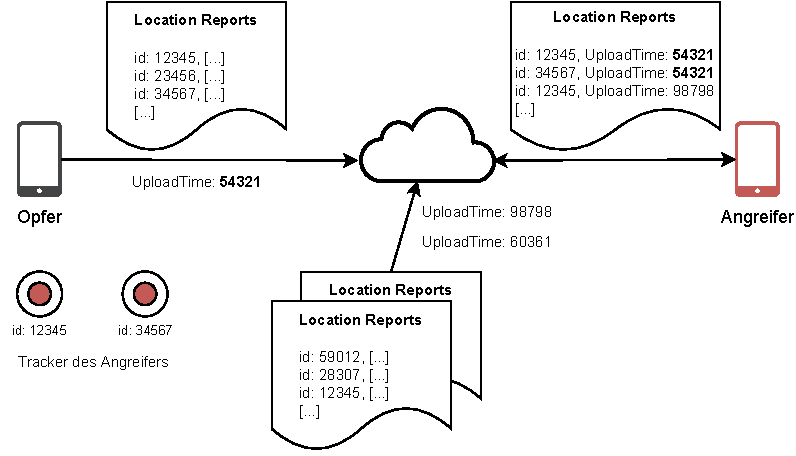
\includegraphics[width=0.9\textwidth]{indirektes_tracking.pdf}
  \caption{Schema zum indirekten Tracking von Personen.}
  \label{fig:indirect_tracking}
\end{figure}

Zur Nutzung als Tool für das Crowd-Monitoring werden einzelne Tracker an öffentlichen Orten platziert.
Finder Devices, die sich in der Nähe dieser Tracker befinden, generieren Location Reports und laden diese hoch.
Diese Reports können von Apples Servern heruntergeladen werden und erlauben Rückschlüsse über die Anzahl der iPhone-Nutzer, welche sich zu einem bestimmten Zeitpunkt in der Nähe eines Ortes aufgehalten haben.
Dazu werden die Erstellungszeitpunkte der Reports und die Anzahl der Reports für einen bestimmten Tracker herangezogen.
Die Zahl der iPhone-Nutzer kann weiterhin verwendet werden, um die Gesamtzahl der Personen zu schätzen.
Durch die Verzögerung beim Upload der Reports sind die Daten allerdings nur mit einer gewissen Verzögerung verfügbar \cite{Tonetto_FindMy}.

Über die Verwendung mehrerer Tracker lassen sich weiterhin die Bewegungen von Menschenmengen, der sogenannte Crowd-Flow, rekonstruieren.
Dabei werden die Tracker an verschiedenen Orten platziert und die Location Reports der Finder Devices heruntergeladen.
Anhand der Uploadzeitpunkte der Reports kann bestimmt werden, welche Reports vom gleichen Finder Device stammen \cite{Tonetto_FindMy}.
Darauf aufbauend kann die Zeit bestimmt werden, die das Finder Device benötigt hat, die Distanz zwischen jeweils zwei Trackern zurückzulegen.
Alternativ könnte, über das oben vorgestellte Verfahren, die Anzahl der Personen in der Nähe jedes Trackers zu verschiedenen Zeiten bestimmt werden und auf Basis der Veränderungen Rückschlüsse auf die Bewegungen der Menschenmengen gezogen werden.


Dieser Missbrauch des „Wo ist?“ Dienstes kann als Alternative zu aktuellen Crowd-Monitoring-Systemen, welche auf Bilderkennung oder der Auswertung von Wi-Fi Management Frames basieren, verwendet werden und erlaubt eine ähnliche Genauigkeit bei geringerem Eingriff in die Privatsphäre der betroffenen Personen.
Zusätzlich ist dieser Ansatz besser für die Privatsphäre der Betroffenen, da keine personenbezogenen Daten erhoben werden \cite{Tonetto_FindMy}.
Deshalb wird dieser Einsatzzweck als „positiver“ Missbrauch des „Wo ist?“ Dienstes bewertet.


\subsubsection{Gegenmaßnahmen}
Da hier sowohl positive als auch negative Einsatzzwecke möglich sind, sind Gegenmaßnahmen wünschenswert, welche den positiven Nutzen erhalten und gleichzeitig die mögliche negative Nutzung verhindern.
Der negative Missbrauch beruht darauf, mehrere Location Reports eines Finder Devices anhand der Upload-Zeitstempel miteinander in Verbindung zu bringen.
Tonetto \textit{et al.} \cite{Tonetto_FindMy} schlagen daher eine Reduktion der Genauigkeit der Zeitstempel oder deren komplette Abschaffung als Gegenmaßnahmen vor.
Alternativ könnte auch der Upload der einzelnen Location Reports zufällig verteilt werden.
Konkret werden zufällige Zeitintervalle oder zufällige, seit der Erstellung zurückgelegte Distanzen vorgeschlagen.

Diese Maßnahmen sind geeignet, die Zuordnung mehrerer Location Reports zu einem Finder Device zumindest zu erschweren.
Insbesondere durch die komplette Abschaffung der Zeitstempel kann der negative Missbrauch zuverlässig verhindert werden.

Der positive Missbrauch zum Crowd-Monitoring wird durch diese Gegenmaßnahmen nicht komplett verhindert.
Die Abschätzung von Personendichten ist nicht davon abhängig, mehrere Location Reports zu einem Gerät zuzuordnen, sondern nur davon, mehrere Location Reports abrufen zu können.
Die Bestimmung des Crowd-Flows, nach der in \cite{Tonetto_FindMy} vorgestellten Methode, ist hingegen auf diese Zuordnung angewiesen.
Allerdings ließe sich der Crowd-Flow auch anhand der Veränderung der Personendichte über die Zeit abschätzen.
Die Genauigkeit dieser Alternativen Lösung ist mangels Untersuchung durch die Autoren nicht bekannt.
Sofern die Möglichkeit mehrere Location Reports abzurufen nicht eingeschränkt wird, ist der positive Missbrauch weiterhin möglich.
Da durch die Limitierung der Anzahl der Location Reports vermutlich die Genauigkeit der Standortinformationen reduziert werden würde, ist nicht zu erwarten, dass Apple diese Maßnahme umsetzt.

Die Nutzer können sich sowohl gegen positiven als auch negativen Missbrauch nur schwer schützen.
Durch regelmäßige Verbindung mit einem WLAN-Netzwerk wäre es möglich, die Anzahl der zu einem Gerät zuordenbaren Location Reports zu reduzieren, was die negative Ausnutzung erschweren würde.
Jedoch ist die Verbindung mit einem WLAN-Netzwerk nicht immer möglich und auch nicht immer gewünscht.
Geeignete Schutzmaßnahmen müssen demnach von Apple getroffen werden.


\subsection[M5]{M5: Verdeckter Datentransfer}
\label{missbrauch:5}
Tonetto \textit{et al.} \cite{Tonetto_FindMy} und Bräunlein \cite{braeunlein_sendmy} zeigen unabhängig voneinander, dass der „Wo ist?“ Dienst auch für einen verdeckten Datentransfer mit einer niedrigen Übertragungsrate ausgenutzt werden kann.
Dabei werden Finder Devices dazu genutzt, Daten an Apples Server zu übertragen, welche vom Angreifer heruntergeladen und dekodiert werden können.
Beide verwenden für das Senden der Daten inoffizielle Tracker, um die Daten in den Advertisements zu senden.
Der verdeckte Datentransfer kann dem Angreifermodell des Angreifers in der Nähe (A2 in \autoref{fig:adversary_models}) zugeordnet werden.
Allerdings muss das Angreifermodell um das Ziel eines kostenfreien und unentdeckten Datentransfers und der Möglichkeit die Location Reports über die \acp{API} des Diensts herunterzuladen erweitert werden.


Bräunlein \cite{braeunlein_sendmy} kodiert eine zu sendende Nachricht in den öffentlichen Schlüssel, der in Advertisement-Paketen übertragen wird.
Für jedes Bit der Nachricht wird ein 28 Byte langes Array, bestehend aus der Position des Bits in der Nachricht, einer ID des Senders und dem Wert des Bits generiert.
Anstatt einen öffentlichen Schlüssel im Advertisement zu senden, werden die so kodierten Daten für eine definierte Zeitspanne gesendet.
Danach wird der Prozess für das nächste Bit der Nachricht wiederholt.
Diese Kodierung ist in \autoref{fig:sendmy_encoding} schematisch dargestellt.
\begin{figure}[ht]
  \centering
  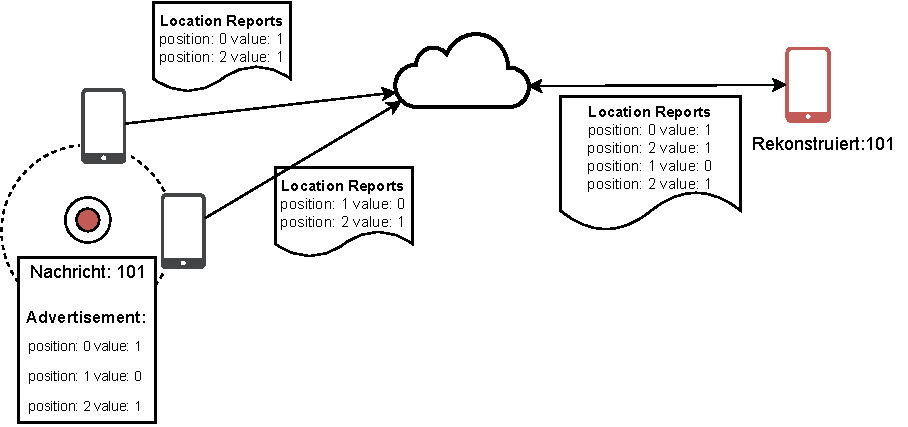
\includegraphics[width=0.95\textwidth]{sendmy.pdf}
  \caption{Bitweise Kodierung einer Nachricht in Advertisement-Pakete, wie von Bräunlein vorgeschlagen.}
  \label{fig:sendmy_encoding}
\end{figure}
Der Empfänger kann für jedes Bit der Nachricht die zwei möglichen Arrays generieren und eine Anfrage mit den jeweiligen \ac{SHA}-256 Hashes an Apples Server senden.
Da jedoch nur ein öffentlicher Schlüssel erzeugt wird, können mit diesen Schlüsseln verschlüsselte Nachrichten nicht entschlüsselt werden.
Jedoch ist für diesen Missbrauch die Entschlüsselung der Daten nicht notwendig, da lediglich das Vorhandensein eines bestimmten Location Reports überprüft werden muss, um die Nachricht zu dekodieren.
Abhängig davon, welcher der beiden Hashes in der Antwort enthalten ist, kann der Empfänger das Bit der Nachricht bestimmen.
Dabei wird ausgenutzt, dass jedes Apple Gerät die verschlüsselten Location Reports für beliebige öffentliche Schlüssel herunterladen kann \cite{Heinrich_OpenHaystack,braeunlein_sendmy}.
Da die Location Reports Ende-zu-Ende verschlüsselt sind, wird dadurch die Vertraulichkeit nicht gefährdet.
Ein Nachteil bei diesem Verfahren ist, dass somit theoretisch jedes Apple-Gerät die Nachricht abrufen könnte.

\begin{figure}[ht]
  \centering
  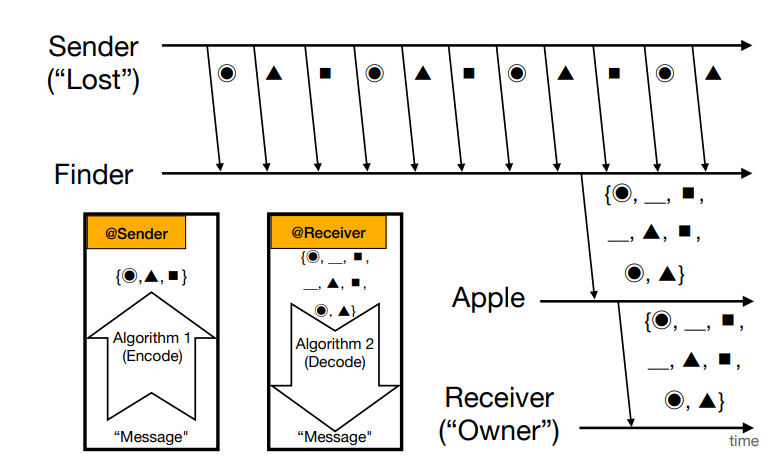
\includegraphics[width=0.7\textwidth]{tagcomm.png}
  \caption{Kodierung einer Nachricht in eine Folge bekannter Advertising Keys, wie von Tonetto \textit{et al.} vorgeschlagen \cite{Tonetto_FindMy}.}
  \label{fig:tagcomm_encoding}
\end{figure}
Das von Tonetto \textit{et al.} \cite{Tonetto_FindMy} vorgestellte Verfahren verwendet stattdessen 16 bekannte Advertising Keys, um die Nachricht in eine Folge dieser Keys zu kodieren.
Dazu wird eine Menge von Advertising Keys zuvor generiert und zwischen Sender und Empfänger ausgetauscht.
Das Verfahren ist in \autoref{fig:tagcomm_encoding} schematisch dargestellt.
Zunächst erzeugt der Sender aus der Nachricht eine Abfolge der Advertising Keys.
Diese werden in dieser Reihenfolge nacheinander in den Advertisement-Paketen gesendet.
Finder Devices, die sich in der Nähe befinden, empfangen die Advertisement-Pakete, erstellen Location Reports und laden diese hoch.
Der Empfänger der Nachricht kann alle Location Reports der bekannten Advertising Keys herunterladen.
Da der Empfänger die Location Reports entschlüsseln kann, erhält er die Zeitstempel der Erstellung der Location Reports.
Daraus kann er die Folge der Advertising Keys rekonstruieren und die Nachricht dekodieren.

Im Vergleich zum Verfahren von Bräunlein, werden hier echte Advertising Keys verwendet, sodass die Location Reports entschlüsselt werden können, sodass der Standort des Senders bestimmt werden kann.
Zusätzlich muss der Empfänger weniger Anfragen an Apples Server stellen, da nur 16 unterschiedliche Advertising Keys verwendet werden.
Bräunleins Verfahren benötigt hingegen zwei Anfragen an Apples Server pro übertragenem Bit \cite{braeunlein_sendmy}.


\subsubsection{Gegenmaßnahmen}
Da die Privatsphäre der Nutzer nicht beeinträchtigt wird und die Praxisrelevanz aufgrund geringer Datenrate niedrig ist, sind Gegenmaßnahmen aus Sicht der Nutzer nicht zwingend erforderlich.
Dennoch hat Apple ein berechtigtes Interesse, den kostenlosen Datentransfer über seinen Dienst zu verhindern.
Der verdeckte Datentransfer ist auf die Verwendung von inoffiziellen Trackern angewiesen, weshalb die Maßnahmen gegen inoffizielle Tracker, wie bei den Gegenmaßnahmen zu \autoref{missbrauch:3} beschrieben, diesen Missbrauch sicher verhindern könnten.
Allerdings treffen die bereits beschriebenen Probleme auch hier zu.

Weiterhin schlagen die Autoren von \cite{Tonetto_FindMy} vor, die Anzahl der Location Reports, die von einem Finder Device hochgeladen werden können, zu begrenzen.
Durch andere Finder Devices in der Nähe, reicht diese Begrenzung jedoch nicht aus um den verdeckten Datentransfer zuverlässig zu verhindern.
Zusätzlich könnte die Anzahl der abrufbaren Location Reports pro Advertising Key limitiert werden.
Die Kodierung, wie von Bräunlein \cite{braeunlein_sendmy} vorgeschlagen, wäre davon allerdings nicht betroffen, da für jedes Bit der Nachricht ein eigener Advertising Key verwendet wird und somit nur ein Location Report abrufbar sein muss.

Apple könnte zusätzlich den Abruf von Location Reports auf Lost Devices beschränken, die unter der gleichen Apple-ID registriert sind.
Eine Registrierung, welche die Zuordnung eines hochgeladenen Location Reports zu einer Apple-ID erlaubt, ist jedoch im Dienst aktuell nicht vorgesehen und würde ebenfalls eine signifikante Anpassung des Dienstes erfordern.
Eine Möglichkeit hierzu wäre die Verknüpfung des \ac{MBK} mit der Apple-ID, was die Ende-zu-Ende-Verschlüsselung aufweicht.
Alternativ könnte das Advertisement-Format um Daten zur Verknüpfung mit der Apple-ID erweitert werden.
Letzteres würde die Verfolgbarkeit von Lost Devices anhand der Advertisement-Pakete im Vergleich zum aktuellen System erleichtern.
Zusätzlich bietet bereits die aktuelle Implementierung keine Möglichkeit zusätzliche Daten in den Advertisement-Paketen zu senden.
Apple hat demnach keine Möglichkeit den Missbrauch einzuschränken, ohne signifikante Anpassungen des Dienstes vorzunehmen.



\subsection[M6]{M6: Korrelation von Standorten durch Apple}
\label{missbrauch:6}

Das zweite Ziel im Angreifermodell des Dienstanbieters (A4 in \autoref{fig:adversary_models}) bezieht sich auf die Korrelation von Standorten mehrerer Nutzer.
Heinrich \textit{et al.} \cite{Heinrich_FindMy} zeigen, dass durch den authentifizierten Upload und Download, die Korrelation durch Apple theoretisch möglich ist.
Die konkreten Standorte können aufgrund der Ende-zu-Ende-Verschlüsselung nicht bestimmt werden.
Allerdings kann bestimmt werden, welches Gerät welche Location Reports erstellt und welcher Nutzer diese heruntergeladen hat.
Daraus lässt sich folgern, welche Nutzer sich zu welcher Zeit an einem gemeinsamen Ort aufgehalten haben.
Apple könnte diese Informationen für eigene Zwecke nutzen, zum Beispiel um soziale Beziehungen zwischen Nutzern für personalisierte Werbung zu analysieren.
In \cite{Heinrich_FindMy} wird zusätzlich gezeigt, dass diese Daten auch von Strafverfolgungsbehörden genutzt werden könnten, um beispielsweise die Identität von Demonstrationsteilnehmern zu bestimmen.

Zumindest nach US-Recht existieren verschiedene Möglichkeiten für Strafverfolgungsbehörden, von Apple gespeicherte Daten anzufragen \cite{Data_Access}.
In den „Richtlinien für Rechtsverfahren [für] Regierungs- und Strafverfolgungsbehörden außerhalb der USA“ \cite{Apple_FindMy_Data} gibt Apple an, dass aufgrund der Verschlüsselung kein Zugriff auf die Standortdaten der Nutzer möglich ist.
Allerdings stehen „Verbindungsprotokolle zu ‚Wo ist?’ [stehen] für einen Zeitraum von bis zu 25 Tagen zur Verfügung“ \cite{Apple_FindMy_Data}.
Um diese Verbindungsprotokolle zu erstellen, muss eine Zuordnung von Verbindungen zu Nutzern stattfinden.
Da Verbindungen zum „Wo ist?“ Dienst nur beim Upload oder Download von Location Reports entstehen, kann davon ausgegangen werden, dass Apple diese Daten speichert.
Mit den Daten zur Authentifizierung kann Apple alle Location Report zu bestimmten Nutzern zuordnen.
Das hier beschriebene Szenario ist dadurch auch praktisch umsetzbar und könnte bei entsprechendem Zugriff nicht nur von Apple, sondern auch von Strafverfolgungsbehörden genutzt werden.


\subsubsection{Gegenmaßnahmen}
Um die Korrelation der Standortdaten zu verhindern, muss entweder der Upload oder der Download der Location Reports ohne Authentifizierung erfolgen.
Ein nicht authentifizierter Upload würde jedoch den Upload gefälschter von Location Reports erleichtern, da dafür kein Apple-Gerät mehr benötigt würde.
Die Auswirkungen gefälschter Reports sind mit den Auswirkungen von Replay-Angriffen nach Szenario \nameref{missbrauch:1} vergleichbar und könnten die Verfügbarkeit und Integrität der Standortdaten gefährden.

Der Download könnte prinzipiell ohne Authentifizierung erfolgen, da die Location Reports Ende-zu-Ende-verschlüsselt sind.
Auch die aktuelle Implementierung kann nicht prüfen, ob ein Location Report zur Apple-ID gehört, die den Download anfordert.
Diese Maßnahme wird auch von Heinrich \textit{et al.} \cite{Heinrich_FindMy} vorgeschlagen.
Es wäre jedoch möglich, dass Gegenmaßnahmen für andere Missbrauchsszenarien, wie zum Beispiel \nameref{missbrauch:3} und \nameref{missbrauch:4}, einen authentifizierten Download erforderlich machen.
Weiterhin ist fraglich, inwieweit Apple ein Interesse daran hat, die Korrelation der Standorte der Nutzer zu verhindern.
Es ist aktuell nicht bekannt, ob Apple dieses Missbrauchsszenario für eigene Zwecke nutzt.
Auch ist nicht klar, ob und wie häufig Strafverfolgungsbehörden die Daten zu „Wo ist?“ anfragen, da diese Informationen in Apples Transparenzbericht nicht gesondert aufgeführt werden \cite{Apple_Transparency}.

Es sind weiterhin keine Maßnahmen bekannt, wie Nutzer diesen Missbrauch verhindern oder erschweren können.
